\documentclass[12pt,addpoints]{repaso}
\grado{1}
\nivel{Secundaria}
\cicloescolar{2024-2025}
\materia{Matemáticas 1 \normalfont \color{darkgray} \\[-0.2em] \small con adecuación curricular a Matemáticas 4$^\circ$ de Primaria}
\unidad{1, 2 y 3}
\title{Practica la Unidad}
\aprendizajes{%
      \item hola
}
\author{Melchor Pinto, JC}
\begin{document}
\INFO
\begin{questions}
	% UNIDAD 1                  
	% \section*{\ifprintanswers{Escritura de cantidades                        }\else{}\fi}
	% \subsection*{\ifprintanswers{Escritura de cantidades 1                      }\else{}\fi}

	% \questionboxed[6]{Escribe los siguientes números

	% 	\begin{multicols}{3}
	% 		\begin{parts}
	% 			\part Setecientos doce
	% 			\part Ochocientos noventa y seis
	% 			\part Setecientos treinta y dos
	% 			\part Setecientos sesenta y dos
	% 			\part Ochocientos noventa
	% 			\part Setecientos setenta
	% 			\part Setecientos tres
	% 			\part Seiscientos noventa y dos
	% 			\part Novecientos treinta y tres
	% 			\part Ochocientos veintiuno
	% 			\part Novecientos cincuenta y seis
	% 			\part Ochocientos cincuenta
	% 			\part Setecientos noventa y tres
	% 			\part Ochocientos setenta y cuatro
	% 			\part Seiscientos cincuenta y tres
	% 		\end{parts}
	% 	\end{multicols}
	% }

	% \subsection*{\ifprintanswers{Escritura de cantidades 2                      }\else{}\fi}
	% \questionboxed[6]{Escribe los siguientes números

	% 	\begin{multicols}{3}
	% 		\begin{parts}
	% 			\part Mil novecientos
	% 			\part Mil seiscientos tres
	% 			\part Mil quinientos ochenta y ocho
	% 			\part Mil quinientos
	% 			\part Mil novecientos treinta y dos
	% 			\part Mil novecientos cincuenta y dos
	% 			\part Mil ochocientos cuarenta y nueve
	% 			\part Mil trescientos diez
	% 			\part Mil quinientos sesenta
	% 			\part Mil novecientos sesenta
	% 			\part Mil doscientos
	% 			\part Mil ochocientos cincuenta y seis
	% 			\part Mil novecientos veinticinco
	% 			\part Mil noventa y tres
	% 			\part Mil trescientos cuarenta y cinco
	% 		\end{parts}
	% 	\end{multicols}
	% }

	% \subsection*{\ifprintanswers{Escritura de cantidades 3                      }\else{}\fi}
	% \questionboxed[6]{Escribe los siguientes números

	% 	\begin{multicols}{3}
	% 		\begin{parts}
	% 			\part Dos mil doscientos ocho
	% 			\part Dos mil setecientos noventa y uno
	% 			\part Dos mil setenta y cuatro
	% 			\part Dos mil quince
	% 			\part Cuatro mil ochenta y ocho
	% 			\part Tres mil trescientos treinta y tres
	% 			\part Tres mil setecientos sesenta y dos
	% 			\part Cuatro mil cuarenta y cuatro
	% 			\part Dos mil seiscientos
	% 			\part Tres mil trescientos ochenta y nueve
	% 			\part Tres mil novecientos sesenta y seis
	% 			\part Cuatro mil cuatrocientos
	% 			\part Dos mil trescientos quince
	% 			\part Cuatro mil trescientos sesenta y ocho
	% 			\part Dos mil ochenta y nueve
	% 		\end{parts}
	% 	\end{multicols}
	% }

	% \subsection*{\ifprintanswers{Escritura de cantidades 4                      }\else{}\fi}
	% \questionboxed[6]{Escribe los siguientes números

	% 	\begin{multicols}{3}
	% 		\begin{parts}
	% 			\part Siete mil doscientos sesenta y nueve    \fillin[7269][0in]
	% 			\part Siete mil ciento treinta y nueve    \fillin[7139][0in]
	% 			\part Ocho mil doscientos cincuenta y nueve    \fillin[8259][0in]
	% 			\part Seis mil setecientos cuarenta y cuatro    \fillin[6744][0in]
	% 			\part Siete mil seiscientos setenta y uno    \fillin[7671][0in]
	% 			\part Nueve mil doscientos cincuenta y cinco    \fillin[9255][0in]
	% 			\part Siete mil    \fillin[7000][0in]
	% 			\part Siete mil ciento treinta y seis    \fillin[7136][0in]
	% 			\part Ocho mil ciento cincuenta y cuatro    \fillin[8154][0in]
	% 			\part Cinco mil trescientos sesenta y seis    \fillin[5366][0in]
	% 			\part Siete mil cuatrocientos ochenta y uno    \fillin[7481][0in]
	% 			\part Ocho mil novecientos noventa y cinco    \fillin[8995][0in]
	% 			\part Seis mil doscientos veintidos    \fillin[6222][0in]
	% 			\part Cinco mil doscientos veintisiete    \fillin[5227][0in]
	% 			\part Siete mil setecientos setenta y siete    \fillin[7777][0in]
	% 		\end{parts}
	% 	\end{multicols}
	% }
	% \subsection*{\ifprintanswers{Escritura de cantidades 5                      }\else{}\fi}
	\questionboxed[6]{Escribe los siguientes números

		\begin{multicols}{2}
			\begin{parts}
				\part Catorce mil cinco.                         \\ \hfill \fillin[$14005$][2cm]
				\part Once mil quinientos noventa y cuatro.      \\ \hfill \fillin[$11594$][2cm]
				\part Trece mil seiscientos cuarenta y cuatro.   \\ \hfill \fillin[$13644$][2cm]
				\part Diez mil ciento ochenta y nueve.           \\ \hfill \fillin[$10189$][2cm]
				\part Trece mil novecientos noventa y nueve.     \\ \hfill \fillin[$13999$][2cm]
				\part Once mil trescientos.                      \\ \hfill \fillin[$11300$][2cm]
				\part Catorce mil cuatrocientos.                 \\ \hfill \fillin[$14400$][2cm]
				\part Doce mil ochocientos ochenta y uno.        \\ \hfill \fillin[$12881$][2cm]
				\part Diez mil setecientos once.                 \\ \hfill \fillin[$10711$][2cm]
				\part Once mil setecientos cuarenta y nueve.     \\ \hfill \fillin[$11749$][2cm]
				\part Diez mil doscientos noventa y ocho.        \\ \hfill \fillin[$10298$][2cm]
				\part Diez mil cuatrocientos cincuenta y siete.  \\ \hfill \fillin[$10456$][2cm]
				\part Trece mil cuatrocientos veintidos.         \\ \hfill \fillin[$13422$][2cm]
			\end{parts}
		\end{multicols}
	}
	% \section*{\ifprintanswers{Números romanos                                }\else{}\fi}
	% \subsection*{\ifprintanswers{Números romanos 1                              }\else{}\fi}
	% \subsection*{\ifprintanswers{Números romanos 2                              }\else{}\fi}
	% \subsection*{\ifprintanswers{Números romanos 3                              }\else{}\fi}
	% \subsection*{\ifprintanswers{Números romanos 4                              }\else{}\fi}
	% \subsection*{\ifprintanswers{Números romanos 5                              }\else{}\fi}
	\questionboxed[6]{Escribe el valor de los siguientes números romanos

		\begin{multicols}{3}
			\begin{parts}
				\part XVI       \fillin[$14005$][2cm]
				\part CDLXXXII  \fillin[$14005$][2cm]
				\part XVIII     \fillin[$14005$][2cm]
				\part XCVIII    \fillin[$14005$][2cm]
				\part LXIV      \fillin[$14005$][2cm]
				\part CXCIX     \fillin[$14005$][2cm]
				\part XXXVI     \fillin[$14005$][2cm]
				\part XLII      \fillin[$14005$][2cm]
				\part XXXVII    \fillin[$14005$][2cm]
				\part LXIII     \fillin[$14005$][2cm]
				\part XXIX      \fillin[$14005$][2cm]
				\part XXXIV     \fillin[$14005$][2cm]
			\end{parts}
		\end{multicols}
	}

	\questionboxed[6]{Escribe en números romanos los siguientes números

		\begin{multicols}{3}
			\begin{parts}
				\part 38  \fillin[$14005$][2cm]
				\part 150 \fillin[$14005$][2cm]
				\part 82  \fillin[$14005$][2cm]
				\part 199 \fillin[$14005$][2cm]
				\part 46  \fillin[$14005$][2cm]
				\part 98  \fillin[$14005$][2cm]
				\part 482 \fillin[$14005$][2cm]
				\part 28  \fillin[$14005$][2cm]
				\part 45  \fillin[$14005$][2cm]
				\part 94  \fillin[$14005$][2cm]
				\part 308 \fillin[$14005$][2cm]
				\part 40  \fillin[$14005$][2cm]
			\end{parts}
		\end{multicols}
	}

	% \section*{\ifprintanswers{Sistema decimal                                }\else{}\fi}
	% \subsection*{\ifprintanswers{Posicionamiento decimal 1                      }\else{}\fi}
	% \subsection*{\ifprintanswers{Posicionamiento decimal 2                      }\else{}\fi}

	\questionboxed[6]{Señala la opción que responda correctamente a cada una de las siguientes preguntas:

		\begin{multicols}{2}
			\begin{parts}
				% \part ¿Qué lugar ocupa el 5 en el número 15484?    \fillin[C][2cm]  
				\part ¿Qué lugar ocupa el 6 en el número 6418?     \fillin[C][1cm]
				% \part ¿Qué lugar ocupa el 3 en el número 3265?  \fillin[C][2cm]
				\part ¿Qué lugar ocupa el 2 en el número 206418?   \fillin[A][1cm]
				\part ¿Qué lugar ocupa el 2 en el número 87264?    \fillin[D][1cm]
				\part ¿Qué lugar ocupa el 1 en el número 1681?     \fillin[F][1cm]
				\part ¿Qué lugar ocupa el 1 en el número 6138?     \fillin[D][1cm]
				\part ¿Qué lugar ocupa el 8 en el número 198114?   \fillin[C][1cm]
				\part ¿Qué lugar ocupa el 7 en el número 46878?    \fillin[E][1cm]
				% \part ¿Qué lugar ocupa el 3 en el número 8131?   \fillin[E][2cm]
				% \part ¿Qué lugar ocupa el 1 en el número 35418?  \fillin[E][2cm] 
				\part ¿Qué lugar ocupa el 4 en el número 149778?  \fillin[B][1cm]
				% \part ¿Qué lugar ocupa el 6 en el número 9167?   \fillin[E][2cm]
				% \part ¿Qué lugar ocupa el 9 en el número 49778?  \fillin[C][2cm]
				% \part ¿Qué lugar ocupa el 6 en el número 6984?   \fillin[C][2cm]
			\end{parts}

			\columnbreak%

			\begin{choices}
				\choice centenas de millar
				\choice decenas de millar
				\choice unidades de millar
				\choice centenas
				\choice decenas
				\choice unidades
			\end{choices}
		\end{multicols}
	}

	% \subsection*{\ifprintanswers{Notación desarrollada 1                        }\else{}\fi}
	% \subsection*{\ifprintanswers{Notación desarrollada 2                        }\else{}\fi}


	\questionboxed[6]{Escribe la notación desarrollada de cada uno de los siguientes números:

		\begin{multicols}{3}
			\begin{parts}
				\part 15984   \fillin[$10000+5000+900+80+4$][0.6in]
				\part 4936    \fillin[$4000+900+30+6$][0.6in]
				\part 27545   \fillin[$20000+7000+500+40+5$][0.6in]
				\part 6215    \fillin[$6000+200+10+5$][0.6in]
				\part 5454    \fillin[$5000+400+50+4$][0.6in]
				\part 6451    \fillin[$6000+400+50+1$][0.6in]
				\part 19679   \fillin[$10000+9000+600+70+9$][0.6in]
				\part 26324   \fillin[$20000+6000+300+20+4$][0.6in]
				\part 5717    \fillin[$5000+700+10+7$][0.6in]
				\part 31126   \fillin[$30000+1000+100+20+6$][0.6in]
				\part 4818    \fillin[$4000+800+10+8$][0.6in]
				\part 7145    \fillin[$7000+100+40+5$][0.6in]
			\end{parts}
		\end{multicols}
	}

	% \subsection*{\ifprintanswers{Posicionamiento decimal y Notación desarrollada}\else{}\fi}

	\questionboxed[6]{Señala la opción que responda correctamente a cada una de las siguientes preguntas:

		\begin{multicols}{2}
			\begin{parts}
				\part En el número 3658, ¿qué número ocupa la posición de las decenas?

				\begin{oneparcheckboxes}
					\choice 3 \choice 5 \choice 6 \choice 8 \choice 9
				\end{oneparcheckboxes}

				\part En el número 17542, ¿qué número ocupa la posición de las unidades de millar?
			
				\begin{oneparcheckboxes}
					\choice 1 \choice 7 \choice 5 \choice 4 \choice 2
				\end{oneparcheckboxes}

				\part En el número 5984, ¿qué número ocupa la posición de las centenas?
				
				\begin{oneparcheckboxes}
					\choice 5 \choice 8 \choice 9 \choice 4 \choice 2
				\end{oneparcheckboxes}
				
				\part En el número 7841, ¿qué número ocupa la posición de las decenas?
				
				\begin{oneparcheckboxes}
					\choice 1 \choice 7 \choice 8 \choice 4 \choice 2
				\end{oneparcheckboxes}
				
				\part En el número 3918, ¿qué número ocupa la posición de las centenas?
				
				\begin{oneparcheckboxes}
					\choice 3 \choice 1 \choice 6 \choice 8 \choice 9
				\end{oneparcheckboxes}

				\part En el número 3621, ¿qué número ocupa la posición de las decenas?
				
				\begin{oneparcheckboxes}
					\choice 3 \choice 2 \choice 6 \choice 8 \choice 1
				\end{oneparcheckboxes}

				\part En el número 51362, ¿qué número ocupa la posición de las decenas de millar?
				
				\begin{oneparcheckboxes}
					\choice 3 \choice 5 \choice 6 \choice 1 \choice 2
				\end{oneparcheckboxes}

				\part En el número 7584, ¿qué número ocupa la posición de las decenas?
				
				\begin{oneparcheckboxes}
					\choice 3 \choice 5 \choice 7 \choice 8 \choice 4
				\end{oneparcheckboxes}

				\part En el número 9654, ¿qué número ocupa la posición de las centenas?
				
				\begin{oneparcheckboxes}
					\choice 3 \choice 5 \choice 6 \choice 4 \choice 9
				\end{oneparcheckboxes}

				\part En el número 240679, ¿qué número ocupa la posición de las centenas de millar?
				
				\begin{oneparcheckboxes}
					 \choice 0 \choice 6 \choice 2 \choice 7 \choice 9 \choice 4
				\end{oneparcheckboxes}
% \part En el número 41589, ¿qué número ocupa la posición de las decenas de millar?
				% \part En el número 8459, ¿qué número ocupa la posición de las centenas?
				% \part En el número 10562, ¿qué número ocupa la posición de las centenas?
				% \part En el número 24781, ¿qué número ocupa la posición de las decenas de millar?
				% \part En el número 7856, ¿qué número ocupa la posición de las decenas?
			\end{parts}
		\end{multicols}
	}


	% \section*{\ifprintanswers{Tablas de multiplicar                          }\else{}\fi}
	% \subsection*{\ifprintanswers{Tabla del 1 y 2                                }\else{}\fi}
	% \subsection*{\ifprintanswers{Tabla del 3 y 4                                }\else{}\fi}
	% \subsection*{\ifprintanswers{Tabla del 5 y 6                                }\else{}\fi}
	% \subsection*{\ifprintanswers{Tabla del 7 y 8                                }\else{}\fi}
	% \subsection*{\ifprintanswers{Tabla del 9 y 10                               }\else{}\fi}
	\questionboxed[6]{Reponde las siguientes tablas de multiplicar:

		\begin{multicols}{4}
			\begin{parts}
				\part $5 \times 9=$ \fillin[$45$][0cm]
				\part $5 \times 6=$ \fillin[$30$][0cm]
				\part $6 \times 8=$ \fillin[$48$][0cm]
				\part $6 \times 9=$ \fillin[$54$][0cm]
				\part $3 \times 6=$ \fillin[$18$][0cm]
				\part $2 \times 7=$ \fillin[$14$][0cm]
				\part $4 \times 7=$ \fillin[$28$][0cm]
				\part $3 \times 8=$ \fillin[$24$][0cm]
				\part $2 \times 9=$ \fillin[$18$][0cm]
				\part $4 \times 4=$ \fillin[$16$][0cm]
				\part $7 \times 7=$ \fillin[$49$][0cm]
				\part $7 \times 5=$ \fillin[$35$][0cm]
				\part $5 \times 4=$ \fillin[$20$][0cm]
				\part $8 \times 7=$ \fillin[$56$][0cm]
				\part $7 \times 6=$ \fillin[$42$][0cm]
				\part $9 \times 7=$ \fillin[$63$][0cm]
			\end{parts}
		\end{multicols}
	}
	\questionboxed[6]{Completa las siguientes tablas de multiplicar:

		\begin{multicols}{4}
			\begin{parts}
				\part \fillin[$6$][0.4cm]$\times 6=36$
				\part $8 \times $\fillin[$9$][0.4cm]$=72$
				\part \fillin[$8$][0.4cm]$\times 8=64$
				\part $9 \times $\fillin[$9$][0.4cm]$=81$
				\part \fillin[$7$][0.4cm]$\times 8=56$
				\part $5 \times $\fillin[$10$][0.4cm]$=50$
				\part \fillin[$8$][0.4cm]$\times 5=40$
				\part $4 \times $\fillin[$8$][0.4cm]$=32$
			\end{parts}
		\end{multicols}
	}
	% UNIDAD 2                  
	% \section*{\ifprintanswers{Números decimales            }\else{}\fi}
	% \subsection*{\ifprintanswers{Posicionamiento decimal      }\else{}\fi}
	% \subsection*{\ifprintanswers{Notación desarrollada        }\else{}\fi}
	% \subsection*{\ifprintanswers{Nombre de decimales          }\else{}\fi}
	

	\questionboxed[6]{Señala la opción que responda correctamente a cada una de las siguientes preguntas:

	\begin{multicols}{2}
		\begin{parts}
			\part En el número 1.829, ¿qué número ocupa la posición de las centésimas?

			\begin{oneparcheckboxes}
				\choice 1 \choice 2 \choice 6 \choice 8 \choice 9
			\end{oneparcheckboxes}

			\part En el número 2.087, ¿qué número ocupa la posición de las décimas?
			
			\begin{oneparcheckboxes}
				\choice 0 \choice 2 \choice 7 \choice 8 \choice 9
			\end{oneparcheckboxes}
			
			\part En el número 5.928, ¿qué número ocupa la posición de las décimas?
			
			\begin{oneparcheckboxes}
				\choice 5 \choice 2 \choice 6 \choice 8 \choice 9
			\end{oneparcheckboxes}
		
			\part En el número 3.284, ¿qué número ocupa la posición de las milésimas?
			
			\begin{oneparcheckboxes}
				\choice 4 \choice 2 \choice 3 \choice 8 \choice 9
			\end{oneparcheckboxes}
		
			\part En el número 1.285, ¿qué número ocupa la posición de las décimas?
			
			\begin{oneparcheckboxes}
				\choice 1 \choice 2 \choice 5 \choice 8 \choice 9
			\end{oneparcheckboxes}
			
			\part En el número 1.823, ¿qué número ocupa la posición de las milésimas?
			
			\begin{oneparcheckboxes}
				\choice 1 \choice 2 \choice 6 \choice 8 \choice 3
			\end{oneparcheckboxes}
		\end{parts}
	\end{multicols}
}

\questionboxed[6]{Escribe los siguientes números

		\begin{multicols}{2}
			\begin{parts}
				\part Veinticinco enteros ocho décimas                  \\ \hfill \fillin[$25.8$][2cm]
				\part Seis enteros cuatrocientos veintiocho milésimas   \\ \hfill \fillin[$6.428$][2cm]
				\part Catorce enteros veintinueve centésimas            \\ \hfill \fillin[$14.29$][2cm]
				\part Cuarenta enteros dos décimas                      \\ \hfill \fillin[$40.2$][2cm]
				\part Tres enteros cincuenta y ocho centésimas          \\ \hfill \fillin[$3.58$][2cm]
				\part Cuatro enteros sesenta y nueve milésimas          \\ \hfill \fillin[$4.069$][2cm] 
				\part Siete enteros cuatro décimas                      \\ \hfill \fillin[$ 7.4$][2cm]
				\part Dos enteros siete décimas                         \\ \hfill \fillin[$2.7$][2cm] 
				\part Cuatro enteros ocho milésimas                     \\ \hfill \fillin[$4.008$][2cm] 
				\part Siete enteros setenta y siete centésimas          \\ \hfill \fillin[$7.77$][2cm] 
				\part Once enteros ochenta y nueve centésimas           \\ \hfill \fillin[$11.89$][2cm] 
				\part Treinta y ocho enteros nueve décimas              \\ \hfill \fillin[$38.9$][2cm]
			\end{parts} 
		\end{multicols}
	}
	
	% \subsection*{\ifprintanswers{Suma de decimales            }\else{}\fi}
	\questionboxed[6]{Realiza las siguientes sumas con números decimales:

		\begin{multicols}{3}
			\begin{parts}
				\part \ifprintanswers{\large  \quad   \opadd[hfactor=decimal,resultstyle=\color{red},carryadd=true,carrysub=false]{5.341}{2.514} \\[1ex]}
				\else{          \large  \quad  \opadd[hfactor=decimal,resultstyle=\color{white},carryadd=false,carrysub=false]{5.341}{2.514} \\[1ex]}
				\fi
				\part \ifprintanswers{\large  \quad   \opadd[hfactor=decimal,resultstyle=\color{red},carryadd=true,carrysub=false]{4.49}{1.27} \\[1ex]}
				\else{          \large  \quad  \opadd[hfactor=decimal,resultstyle=\color{white},carryadd=false,carrysub=false]{4.49}{1.27} \\[1ex]} 
				\fi
				\part \ifprintanswers{\large  \quad   \opadd[hfactor=decimal,resultstyle=\color{red},carryadd=true,carrysub=false]{4.1}{2.5} \\[1ex]}
				\else{          \large  \quad  \opadd[hfactor=decimal,resultstyle=\color{white},carryadd=false,carrysub=false]{4.1}{2.5} \\[1ex]}
				\fi
				\part \ifprintanswers{\large  \quad   \opadd[hfactor=decimal,resultstyle=\color{red},carryadd=true,carrysub=false]{3.19}{1.57} \\[1ex]}
				\else{          \large  \quad  \opadd[hfactor=decimal,resultstyle=\color{white},carryadd=false,carrysub=false]{3.19}{1.57} \\[1ex]}
				\fi
				\part \ifprintanswers{\large  \quad   \opadd[hfactor=decimal,resultstyle=\color{red},carryadd=true,carrysub=false]{4.24}{2.37} \\[1ex]}
				\else{          \large  \quad  \opadd[hfactor=decimal,resultstyle=\color{white},carryadd=false,carrysub=false]{4.24}{2.37} \\[1ex]}
				\fi
				\part \ifprintanswers{\large  \quad   \opadd[hfactor=decimal,resultstyle=\color{red},carryadd=true,carrysub=false]{2.928}{1.714} \\[1ex]}
				\else{          \large  \quad  \opadd[hfactor=decimal,resultstyle=\color{white},carryadd=false,carrysub=false]{2.928}{1.714} \\[1ex]}
				\fi
			\end{parts}
		\end{multicols}
	}

	% \subsection*{\ifprintanswers{Resta de decimales           }\else{}\fi}

	\questionboxed[6]{Realiza las siguientes restas con números decimales:

	\begin{multicols}{3}
		\begin{parts}
			\part \ifprintanswers{\large  \quad   \opsub[hfactor=decimal,resultstyle=\color{red},carryadd=true,carrysub=false]{4.3}{2.4} \\[1ex]}
			\else{          \large  \quad  \opsub[hfactor=decimal,resultstyle=\color{white},carryadd=false,carrysub=false]{4.3}{2.4} \\[1ex]}
			\fi
			\part \ifprintanswers{\large  \quad   \opsub[hfactor=decimal,resultstyle=\color{red},carryadd=true,carrysub=false]{4.33}{2.47} \\[1ex]}
			\else{          \large  \quad  \opsub[hfactor=decimal,resultstyle=\color{white},carryadd=false,carrysub=false]{4.33}{2.47} \\[1ex]} 
			\fi
			\part \ifprintanswers{\large  \quad   \opsub[hfactor=decimal,resultstyle=\color{red},carryadd=true,carrysub=false]{5.81}{5.23} \\[1ex]}
			\else{          \large  \quad  \opsub[hfactor=decimal,resultstyle=\color{white},carryadd=false,carrysub=false]{5.81}{5.23} \\[1ex]}
			\fi
			\part \ifprintanswers{\large  \quad   \opsub[hfactor=decimal,resultstyle=\color{red},carryadd=true,carrysub=false]{4.28}{1.96} \\[1ex]}
			\else{          \large  \quad  \opsub[hfactor=decimal,resultstyle=\color{white},carryadd=false,carrysub=false]{4.28}{1.96} \\[1ex]}
			\fi
			\part \ifprintanswers{\large  \quad   \opsub[hfactor=decimal,resultstyle=\color{red},carryadd=true,carrysub=false]{3.14}{2.47} \\[1ex]}
			\else{          \large  \quad  \opsub[hfactor=decimal,resultstyle=\color{white},carryadd=false,carrysub=false]{3.14}{2.47} \\[1ex]}
			\fi
			\part \ifprintanswers{\large  \quad   \opsub[hfactor=decimal,resultstyle=\color{red},carryadd=true,carrysub=false]{7.24}{3.58} \\[1ex]}
			\else{          \large  \quad  \opsub[hfactor=decimal,resultstyle=\color{white},carryadd=false,carrysub=false]{7.24}{3.58} \\[1ex]}
			\fi
		\end{parts}
	\end{multicols}
}

	% \section*{\ifprintanswers{Sumas                        }\else{}\fi}
	% \subsection*{\ifprintanswers{Sumas sin acarreos 1         }\else{}\fi}
	% \subsection*{\ifprintanswers{Sumas sin acarreos 2         }\else{}\fi}
	% \subsection*{\ifprintanswers{Sumas con acarreos 1         }\else{}\fi}
	% \subsection*{\ifprintanswers{Sumas con acarreos 2         }\else{}\fi}
	% \subsection*{\ifprintanswers{Repaso de sumas              }\else{}\fi}

	\questionboxed[6]{Realiza las siguientes sumas:

		\begin{multicols}{3}
			\begin{parts}
				\part \ifprintanswers{\large  \quad   \opadd[hfactor=decimal,resultstyle=\color{red},carryadd=true,carrysub=false]{475}{39} \\[1ex]}
				\else{          \large  \quad  \opadd[hfactor=decimal,resultstyle=\color{white},carryadd=false,carrysub=false]{475}{39} \\[1ex]}
				\fi
				\part \ifprintanswers{\large  \quad   \opadd[hfactor=decimal,resultstyle=\color{red},carryadd=true,carrysub=false]{475}{39} \\[1ex]}
				\else{          \large  \quad  \opadd[hfactor=decimal,resultstyle=\color{white},carryadd=false,carrysub=false]{475}{39} \\[1ex]}
				\fi
				\part \ifprintanswers{\large  \quad   \opadd[hfactor=decimal,resultstyle=\color{red},carryadd=true,carrysub=false]{475}{39} \\[1ex]}
				\else{          \large  \quad  \opadd[hfactor=decimal,resultstyle=\color{white},carryadd=false,carrysub=false]{475}{39} \\[1ex]}
				\fi
				\part \ifprintanswers{\large  \quad   \opadd[hfactor=decimal,resultstyle=\color{red},carryadd=true,carrysub=false]{475}{39} \\[1ex]}
				\else{          \large  \quad  \opadd[hfactor=decimal,resultstyle=\color{white},carryadd=false,carrysub=false]{475}{39} \\[1ex]}
				\fi
				\part \ifprintanswers{\large  \quad   \opadd[hfactor=decimal,resultstyle=\color{red},carryadd=true,carrysub=false]{475}{39} \\[1ex]}
				\else{          \large  \quad  \opadd[hfactor=decimal,resultstyle=\color{white},carryadd=false,carrysub=false]{475}{39} \\[1ex]}
				\fi
				\part \ifprintanswers{\large  \quad   \opadd[hfactor=decimal,resultstyle=\color{red},carryadd=true,carrysub=false]{475}{39} \\[1ex]}
				\else{          \large  \quad  \opadd[hfactor=decimal,resultstyle=\color{white},carryadd=false,carrysub=false]{475}{39} \\[1ex]}
				\fi
			\end{parts}
		\end{multicols}
	}

	% \section*{\ifprintanswers{Restas                       }\else{}\fi}
	% \subsection*{\ifprintanswers{Restas con múltiplos de 100  }\else{}\fi}
	% \subsection*{\ifprintanswers{Restas con transformación 1  }\else{}\fi}
	% \subsection*{\ifprintanswers{Restas con transformación 2  }\else{}\fi}
	% \subsection*{\ifprintanswers{Restas con ceros intermedios }\else{}\fi}
	% \subsection*{\ifprintanswers{Restas con transformación 3  }\else{}\fi}

	\questionboxed[6]{Realiza las siguientes restas:

		\begin{multicols}{3}
			\begin{parts}
				\part \ifprintanswers{\large  \quad   \opsub[hfactor=decimal,resultstyle=\color{red},carryadd=true,carrysub=false]{475}{39} \\[1ex]}
				\else{          \large  \quad  \opsub[hfactor=decimal,resultstyle=\color{white},carryadd=false,carrysub=false]{475}{39} \\[1ex]}
				\fi
				\part \ifprintanswers{\large  \quad   \opsub[hfactor=decimal,resultstyle=\color{red},carryadd=true,carrysub=false]{475}{39} \\[1ex]}
				\else{          \large  \quad  \opsub[hfactor=decimal,resultstyle=\color{white},carryadd=false,carrysub=false]{475}{39} \\[1ex]}
				\fi
				\part \ifprintanswers{\large  \quad   \opsub[hfactor=decimal,resultstyle=\color{red},carryadd=true,carrysub=false]{475}{39} \\[1ex]}
				\else{          \large  \quad  \opsub[hfactor=decimal,resultstyle=\color{white},carryadd=false,carrysub=false]{475}{39} \\[1ex]}
				\fi
				\part \ifprintanswers{\large  \quad   \opsub[hfactor=decimal,resultstyle=\color{red},carryadd=true,carrysub=false]{475}{39} \\[1ex]}
				\else{          \large  \quad  \opsub[hfactor=decimal,resultstyle=\color{white},carryadd=false,carrysub=false]{475}{39} \\[1ex]}
				\fi
				\part \ifprintanswers{\large  \quad   \opsub[hfactor=decimal,resultstyle=\color{red},carryadd=true,carrysub=false]{475}{39} \\[1ex]}
				\else{          \large  \quad  \opsub[hfactor=decimal,resultstyle=\color{white},carryadd=false,carrysub=false]{475}{39} \\[1ex]}
				\fi
				\part \ifprintanswers{\large  \quad   \opsub[hfactor=decimal,resultstyle=\color{red},carryadd=true,carrysub=false]{475}{39} \\[1ex]}
				\else{          \large  \quad  \opsub[hfactor=decimal,resultstyle=\color{white},carryadd=false,carrysub=false]{475}{39} \\[1ex]}
				\fi
			\end{parts}
		\end{multicols}
	}


	% \section*{\ifprintanswers{Multiplicaciones             }\else{}\fi}
	% \subsection*{\ifprintanswers{Multiplicaciones 1           }\else{}\fi}
	% \subsection*{\ifprintanswers{Multiplicaciones 2           }\else{}\fi}
	% \subsection*{\ifprintanswers{Multiplicaciones con 2 cifras}\else{}\fi}
	% \subsection*{\ifprintanswers{Multiplicaciones con 3 cifras}\else{}\fi}
	% \subsection*{\ifprintanswers{Multiplicaciones con 4 cifras}\else{}\fi}

	\questionboxed[6]{Realiza las siguientes multiplicaciones:

		\begin{multicols}{3}
			\begin{parts}
				\part \ifprintanswers{\large  \quad   \opmul[hfactor=decimal,resultstyle=\color{white},displayintermediary=None]{475}{39} \\[1ex]}
				\else{          \large  \quad  \opmul[hfactor=decimal,resultstyle=\color{white},displayintermediary=None]{475}{39} \\[1ex]}
				\fi
				\part \ifprintanswers{\large  \quad   \opmul[hfactor=decimal,resultstyle=\color{white},displayintermediary=None]{475}{39} \\[1ex]}
				\else{          \large  \quad  \opmul[hfactor=decimal,resultstyle=\color{white},displayintermediary=None]{475}{39} \\[1ex]}
				\fi
				\part \ifprintanswers{\large  \quad   \opmul[hfactor=decimal,resultstyle=\color{white},displayintermediary=None]{475}{39} \\[1ex]}
				\else{          \large  \quad  \opmul[hfactor=decimal,resultstyle=\color{white},displayintermediary=None]{475}{39} \\[1ex]}
				\fi
				\part \ifprintanswers{\large  \quad   \opmul[hfactor=decimal,resultstyle=\color{white},displayintermediary=None]{475}{39} \\[1ex]}
				\else{          \large  \quad  \opmul[hfactor=decimal,resultstyle=\color{white},displayintermediary=None]{475}{39} \\[1ex]}
				\fi
				\part \ifprintanswers{\large  \quad   \opmul[hfactor=decimal,resultstyle=\color{white},displayintermediary=None]{475}{39} \\[1ex]}
				\else{          \large  \quad  \opmul[hfactor=decimal,resultstyle=\color{white},displayintermediary=None]{475}{39} \\[1ex]}
				\fi
				\part \ifprintanswers{\large  \quad   \opmul[hfactor=decimal,resultstyle=\color{white},displayintermediary=None]{475}{39} \\[1ex]}
				\else{          \large  \quad  \opmul[hfactor=decimal,resultstyle=\color{white},displayintermediary=None]{475}{39} \\[1ex]}
				\fi
			\end{parts}
		\end{multicols}
	}

	% \section*{\ifprintanswers{Divisiones                   }\else{}\fi}
	% \subsection*{\ifprintanswers{Divisiones sin residuo 1     }\else{}\fi}
	% \subsection*{\ifprintanswers{Divisiones sin residuo 2     }\else{}\fi}
	% \subsection*{\ifprintanswers{Divisiones sin residuo 3     }\else{}\fi}
	% \subsection*{\ifprintanswers{Divisiones con residuo 1     }\else{}\fi}
	% \subsection*{\ifprintanswers{Divisiones con residuo 2     }\else{}\fi}           
	\questionboxed[6]{Realiza las siguientes divisiones:

		\begin{multicols}{3}
			\begin{parts}
				\part \ifprintanswers{\large\opdiv[period,style=text,hrulewidth=0.2pt,vruleperiod=0.7,hfactor=decimal,resultstyle=\color{red}]{123}{6}}
				\else{          \large  \quad $6 \overline{) \ 123\ }$}  \vspace{1cm}
				\fi

				\part \ifprintanswers{\large\opdiv[period,style=text,hrulewidth=0.2pt,vruleperiod=0.7,hfactor=decimal,resultstyle=\color{red}]{200}{3}}
				\else{          \large  \quad $3 \overline{) \ 200\ }$} \vspace{1cm}
				\fi

				\part \ifprintanswers{\large\opdiv[period,style=text,hrulewidth=0.2pt,vruleperiod=0.7,hfactor=decimal,resultstyle=\color{red}]{399}{8}}
				\else{          \large  \quad $8 \overline{) \ 399\ }$} \vspace{1cm}
				\fi

				\part \ifprintanswers{\large\opdiv[period,style=text,hrulewidth=0.2pt,vruleperiod=0.7,hfactor=decimal,resultstyle=\color{red}]{193}{7}}
				\else{          \large  \quad $7 \overline{) \ 193\ }$} \vspace{1cm}
				\fi

				\part \ifprintanswers{\large\opdiv[period,style=text,hrulewidth=0.2pt,vruleperiod=0.7,hfactor=decimal,resultstyle=\color{red}]{283}{6}}
				\else{          \large  \quad $6 \overline{) \ 283\ }$} \vspace{1cm}
				\fi

				\part \ifprintanswers{\large\opdiv[period,style=text,hrulewidth=0.2pt,vruleperiod=0.7,hfactor=decimal,resultstyle=\color{red}]{432}{9}}
				\else{          \large  \quad $9 \overline{) \ 432\ }$} \vspace{1cm}
				\fi

				\part \ifprintanswers{\large\opdiv[period,style=text,hrulewidth=0.2pt,vruleperiod=0.7,hfactor=decimal,resultstyle=\color{red}]{644}{8}}
				\else{          \large  \quad $8 \overline{) \ 644\ }$} \vspace{1cm}
				\fi

				\part \ifprintanswers{\large\opdiv[period,style=text,hrulewidth=0.2pt,vruleperiod=0.7,hfactor=decimal,resultstyle=\color{red}]{656}{7}}
				\else{          \large  \quad $7 \overline{) \ 656\ }$} \vspace{1cm}
				\fi
			\end{parts}
		\end{multicols}
	}
	% UNIDAD 3                  
	% \section*{\ifprintanswers{Introducción a fracciones                  }\else{}\fi}
	% \subsection*{\ifprintanswers{Clasificación de fracciones                }\else{}\fi}

	\questionboxed[4]{Clasifica las siguientes fracciones en propias, impropias o mixtas:
      
	\begin{multicols}{3}
				\begin{parts}
					  \part $\dfrac{5}{6}$ \fillin[Propia][1in]   
					  \part $5\dfrac{5}{11}$ \fillin[Mixta][1in]  
					  \part $\dfrac{7}{3}$ \fillin[Impropia][1in] 
					  \part $\dfrac{3}{4}$ \fillin[Propia][1in]   
					  \part $1\dfrac{2}{3}$ \fillin[Mixta][1in]   
					  \part $\dfrac{7}{5}$ \fillin[Impropia][1in] 
					  \part $\dfrac{7}{8}$ \fillin[Propia][1in]   
					  \part $3\dfrac{2}{9}$ \fillin[Mixta][1in]   
					  \part $\dfrac{3}{2}$ \fillin[Impropia][1in] 
					  % \part $4\dfrac{1}{4}=$ \fillin[Mixta][1in] 
				\end{parts}
		  \end{multicols}
	}

	% \subsection*{\ifprintanswers{Representación de fracciones}\else{}\fi}
	\questionboxed[4]{Escribe sobre la línea la fracción que representa cada imagen:
	
	\begin{multicols}{3}
				\begin{parts}
					  \part 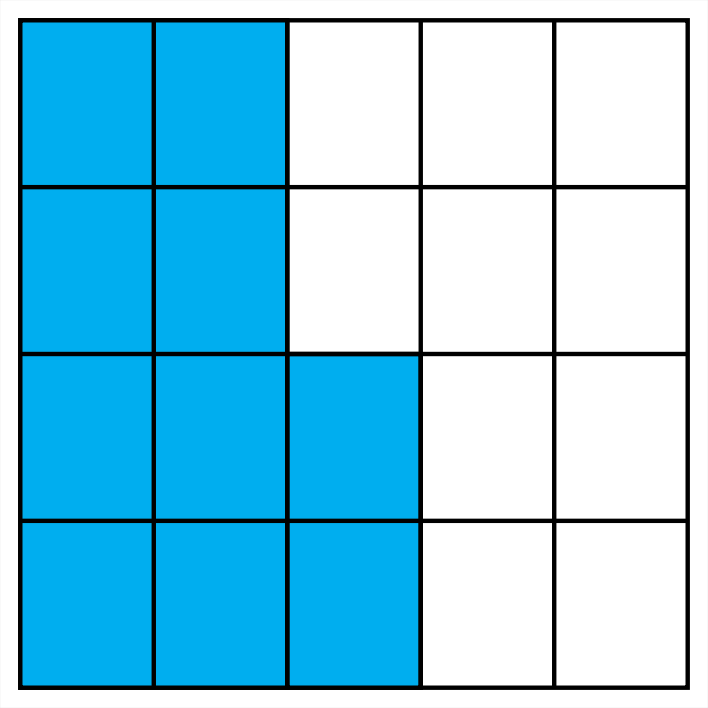
\includegraphics[width=50px]{../images/imagen_frac01.png} \fillin[$\dfrac{10}{20}$][1in]
					  \part 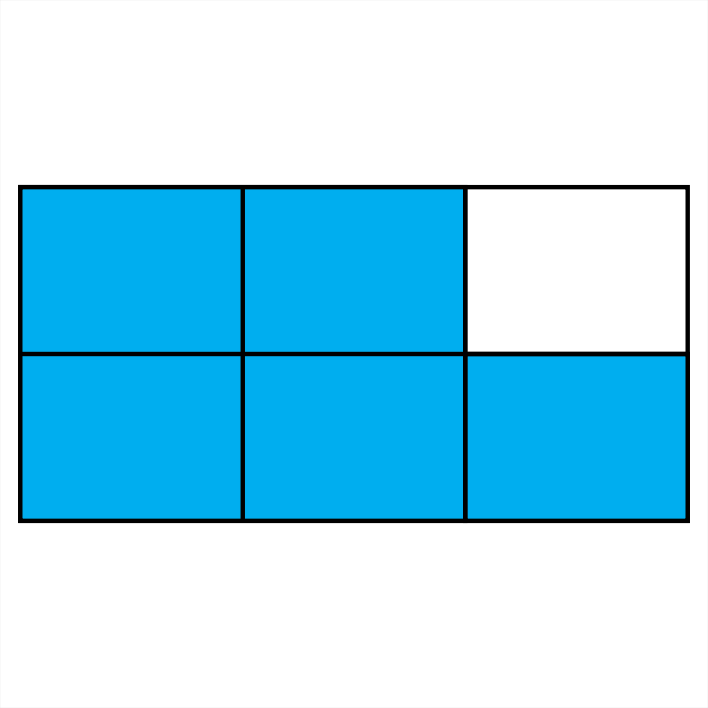
\includegraphics[width=50px]{../images/imagen_frac02.png} \fillin[$\dfrac{5}{6}$][1in]
					  \part 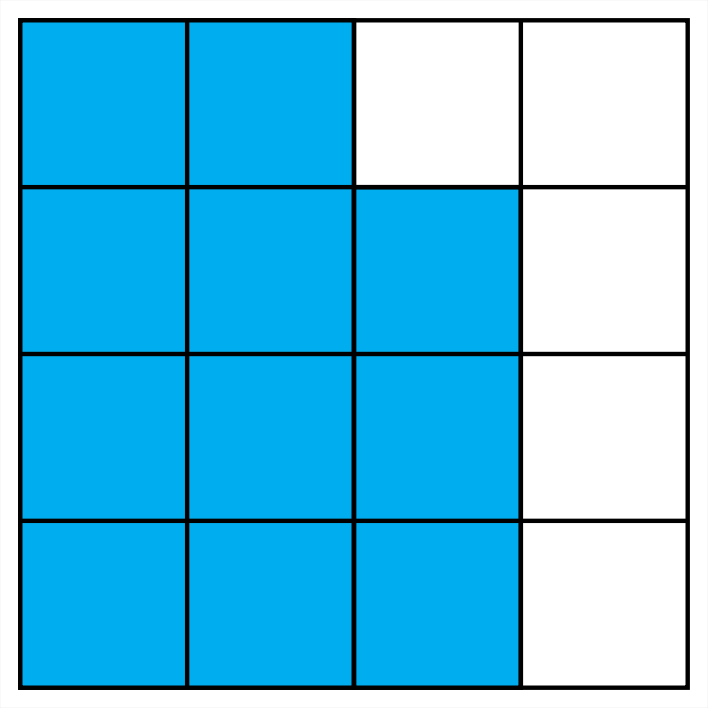
\includegraphics[width=50px]{../images/imagen_frac03.png} \fillin[$\dfrac{11}{16}$][1in]
					  \part 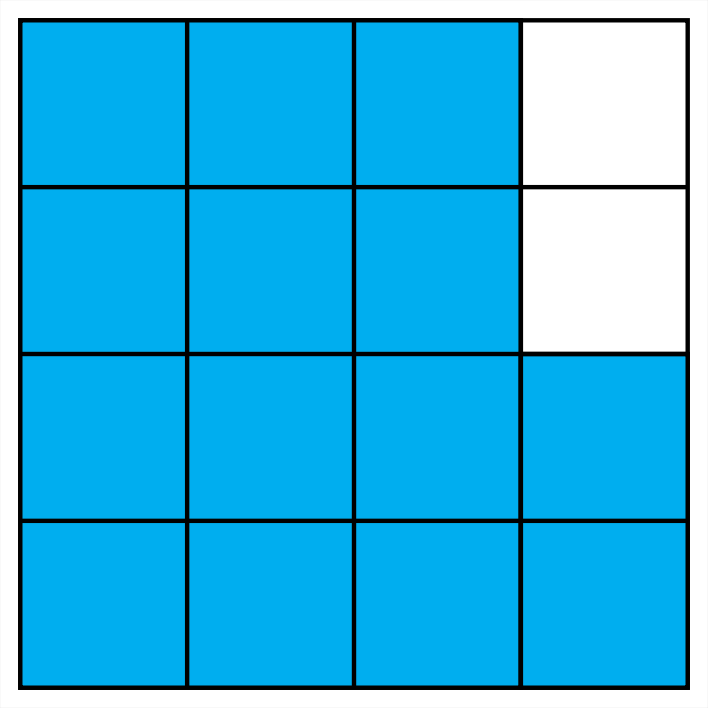
\includegraphics[width=50px]{../images/imagen_frac04.png} \fillin[$\dfrac{14}{16}$][1in]
					  % \part 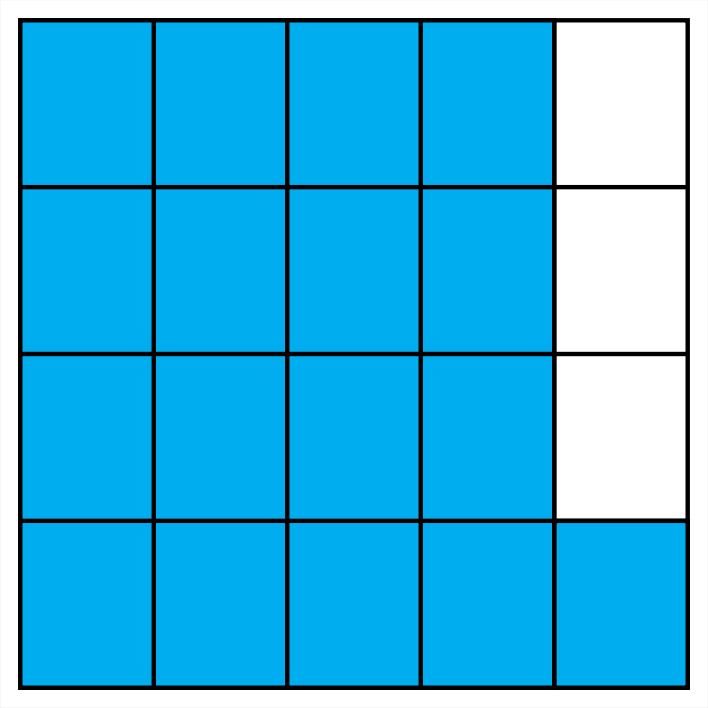
\includegraphics[width=100px]{../images/imagen_frac05.png} \fillin[$\dfrac{10}{20}$][1in]
					  % \part 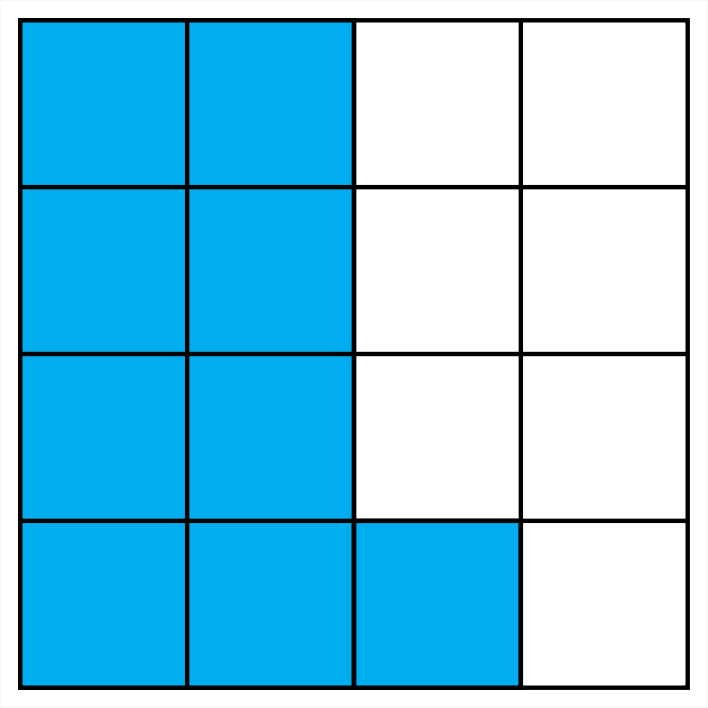
\includegraphics[width=100px]{../images/imagen_frac06.png} \fillin[$\dfrac{10}{20}$][1in]
					  \part 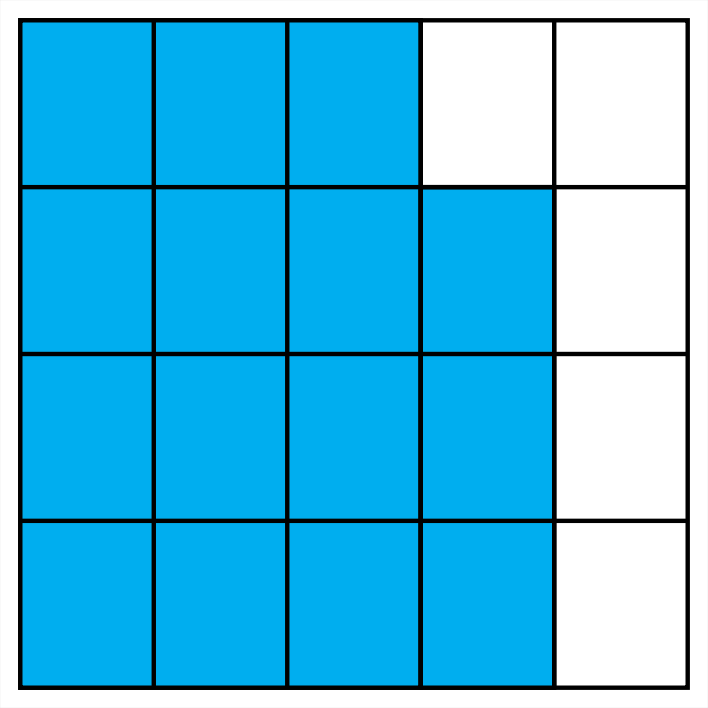
\includegraphics[width=50px]{../images/imagen_frac07.png} \fillin[$\dfrac{15}{20}$][1in]
					  \part 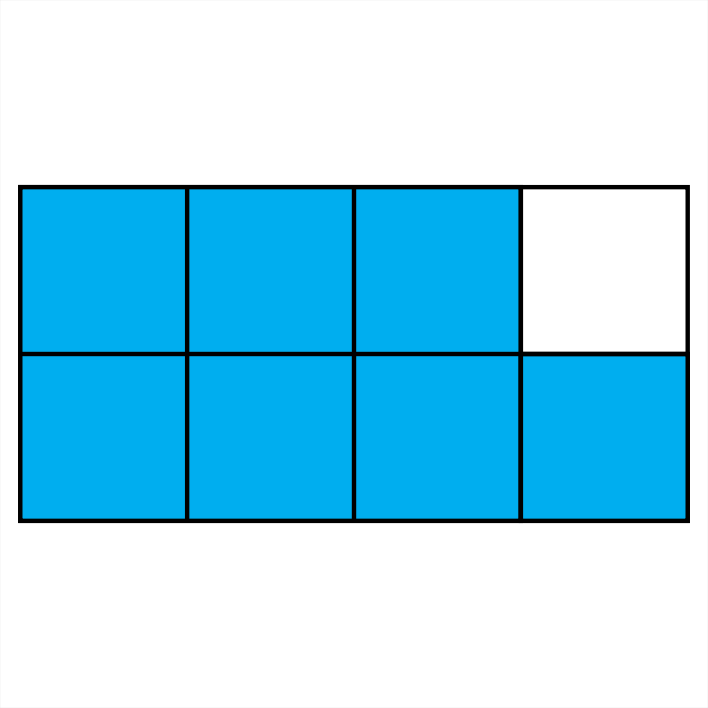
\includegraphics[width=50px]{../images/imagen_frac08.png} \fillin[$\dfrac{7}{8}$][1in]
					  % \part 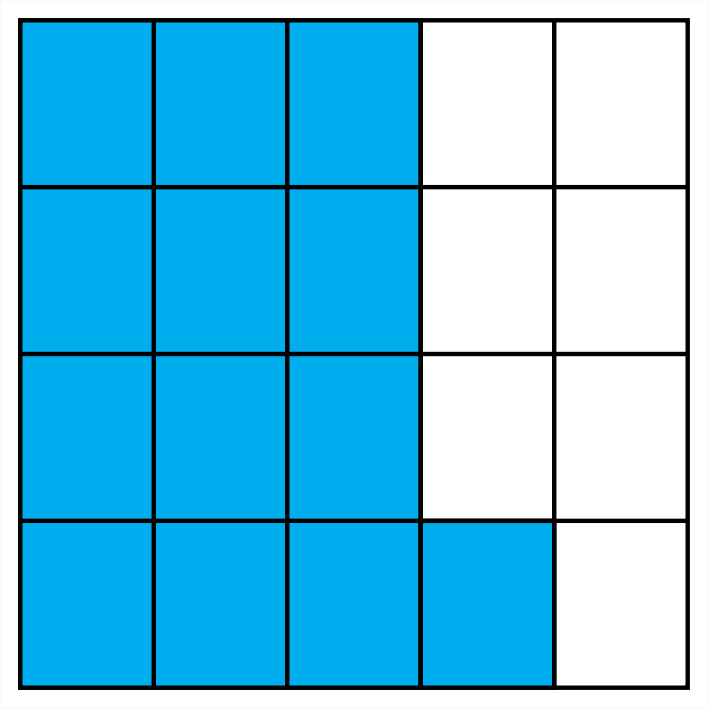
\includegraphics[width=100px]{../images/imagen_frac09.png} \fillin[$\dfrac{10}{20}$][1in]
					  % \part 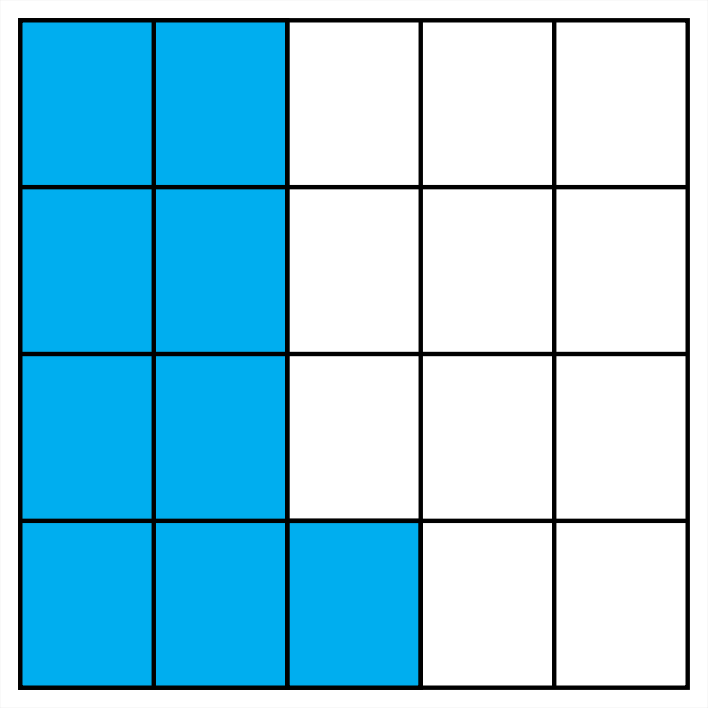
\includegraphics[width=100px]{../images/imagen_frac10.png} \fillin[$\dfrac{10}{20}$][1in]
				\end{parts}
		  \end{multicols}
	}


	% \subsection*{\ifprintanswers{Nombre de fracciones                       }\else{}\fi}
	
	\questionboxed[4]{Escribe la fracción que corresponda en cada inciso:
	\begin{parts}
		  \part ¿Cómo se escribe numéricamente la fracción \textbf{ocho quintos}?    \fillin[$\dfrac{8}{5}$][0in]  \\
		  \part ¿Cómo se escribe numéricamente la fracción \textbf{seis onceavos}?   \fillin[$\dfrac{6}{11}$][0in] \\
		  \part ¿Cómo se escribe numéricamente la fracción \textbf{dos séptimos}?    \fillin[$\dfrac{2}{7}$][0in]  \\
		  \part ¿Cómo se escribe numéricamente la fracción \textbf{once medios}?     \fillin[$\dfrac{11}{2}$][0in] \\
		  \part ¿Cómo se escribe numéricamente la fracción \textbf{diez décimos}?    \fillin[$\dfrac{10}{10}$][0in]\\
	\end{parts}
}

	% \subsection*{\ifprintanswers{Conversión de fracciones mixtas a impropias}\else{}\fi}
	\questionboxed[4]{Convierte la siguientes fracciones mixtas a impropias:
	
	\begin{multicols}{3}
		  \begin{parts}\large
				\part $4\dfrac{2}{3}= $ \fillin[$\dfrac{14}{3}$][0in]
				\part $2\dfrac{3}{10}= $ \fillin[$\dfrac{23}{10}$][0in]
				\part $5\dfrac{1}{5}= $ \fillin[$\dfrac{26}{5}$][0in]
		  \end{parts}
	\end{multicols}
}


	% \subsection*{\ifprintanswers{Conversión de fracciones impropias a mixtas}\else{}\fi}

	\questionboxed[4]{Convierte la siguientes fracciones impropias a mixtas:

	\begin{multicols}{3}
		  \begin{parts}\large
				\part $\dfrac{13}{3}= $ \fillin[$4\dfrac{1}{3}$][0in]
				\part $\dfrac{63}{10}= $ \fillin[$6\dfrac{3}{10}$][0in]
				\part $\dfrac{51}{5}= $ \fillin[$10\dfrac{1}{5}$][0in]
		  \end{parts}
	\end{multicols}
}

	% \section*{\ifprintanswers{Operaciones con fracciones                 }\else{}\fi}
	% \subsection*{\ifprintanswers{Suma de fracciones                         }\else{}\fi}
	% \subsection*{\ifprintanswers{Resta de fracciones                        }\else{}\fi}
	% \subsection*{\ifprintanswers{Multiplicación de fracciones               }\else{}\fi}
	% \subsection*{\ifprintanswers{División de fracciones                     }\else{}\fi}
	% \subsection*{\ifprintanswers{Operaciones de fracciones mixtas           }\else{}\fi}
	
	\questionboxed[15]{Realiza las siguientes operaciones.
	\begin{multicols}{4}
		  \begin{parts}
			    \part $\dfrac{3}{5} \divisionsymbol\dfrac{2}{3}=$ \fillin[$\dfrac{9}{10}$][0.5in] \\[0.75em]
			    \part $\dfrac{7}{8} \divisionsymbol\dfrac{3}{4}=$ \fillin[$\dfrac{28}{24}$][0.5in]	\\[0.75em]		
			    \part $\dfrac{3}{5}\times\dfrac{2}{3}=$ \fillin[$\dfrac{6}{15}$][0.5in]   \\[0.75em]
                \part $\dfrac{7}{8}\times\dfrac{3}{4}=$ \fillin[$\dfrac{21}{32}$][0.5in] \\[0.75em]
				\part $\dfrac{3}{10}+\dfrac{4}{5}=$ \fillin[$\dfrac{11}{10}$ o 1$\dfrac{1}{10}$][0.5in] \\[0.75em]
				\part $\dfrac{3}{4}-\dfrac{2}{5}=$ \fillin[$\dfrac{7}{20}$][0.5in] \\[0.75em]
				\part $\dfrac{2}{3}-\dfrac{2}{5}=$ \fillin[$\dfrac{4}{15}$][0.5in] \\[0.75em]
				\part $\dfrac{3}{8}+\dfrac{7}{10}=$ \fillin[$\dfrac{43}{40}$ o 1$\dfrac{3}{40}$][0.5in] \\[0.75em]
			\end{parts}
		\end{multicols}
  }

	% \section*{\ifprintanswers{Figuras geométricas                        }\else{}\fi}
	% \subsection*{\ifprintanswers{Nombre de figuras                          }\else{}\fi}
	% \subsection*{\ifprintanswers{Elementos de figuras                       }\else{}\fi}
	% \subsection*{\ifprintanswers{Perímetros 1                               }\else{}\fi}
	% \subsection*{\ifprintanswers{Perímetros 2                               }\else{}\fi}
	% \subsection*{\ifprintanswers{Área de figuras                            }\else{}\fi}
	% \section*{\ifprintanswers{Sistema de unidades                        }\else{}\fi}
	% \subsection*{\ifprintanswers{Reloj                                      }\else{}\fi}
	% \subsection*{\ifprintanswers{Multiplicaciones por múltiplos de 10       }\else{}\fi}
	% \subsection*{\ifprintanswers{Unidades de tiempo                         }\else{}\fi}
	% \subsection*{\ifprintanswers{Unidades de longitud                       }\else{}\fi}
	% \subsection*{\ifprintanswers{Unidades de masa                           }\else{}\fi}



\end{questions}
\end{document}